\subsection{PIONEER Goals}
\label{subsec:pioneer-goals}

The primary PIONEER goal considered in this dissertation is a precision
measurement of the charged-pion electron-to-muon decay ratio,
\begin{equation}
  R_{e/\mu}
  =
  \frac{
    \Gamma\!\left(\pi^{+}\to e^{+}\nu_e(\gamma)\right)
  }{
    \Gamma\!\left(\pi^{+}\to \mu^{+}\nu_\mu(\gamma)\right)
  },
  \label{eq:pioneer-goal-remu}
\end{equation}
with a target precision below \(0.01\%\). This observable is the central
Phase-I lepton-flavor-universality measurement in PIONEER. The motivation for
this goal is the mismatch between theoretical and experimental precision. The
Standard Model prediction is
\begin{equation}
  R_{e/\mu}^{\mathrm{SM}}
  =
  1.23524(15)\times 10^{-4},
\end{equation}
whereas the present experimental average is
\begin{equation}
  R_{e/\mu}^{\mathrm{exp}}
  =
  1.23270(230)\times 10^{-4}.
\end{equation}
The world average is dominated by the PIENU result and is tabulated by the
Particle Data Group \cite{pienu_2015,particle_data_group_2024}. The two values
are statistically consistent, but the experimental uncertainty is approximately
a factor of fifteen larger than the theoretical uncertainty
\cite{cirigliano_rosell_2007,pioneer_rare_2022}. PIONEER is designed to reduce
the experimental uncertainty by approximately a factor of fifteen, bringing the
measurement into the same precision regime as the Standard Model calculation.

\begin{figure}[t]
  \centering
  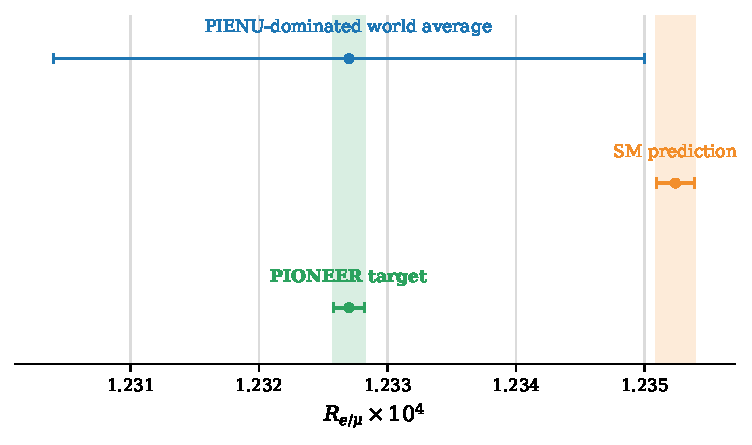
\includegraphics[width=0.75\textwidth]{../resources/figures/generated/pioneer_goal_comparison}
  \caption{
    Current experimental precision and projected PIONEER Phase-I precision for
    \(R_{e/\mu}\). The current world average is taken from the Particle Data
    Group and is dominated by the PIENU measurement
    \cite{pienu_2015,particle_data_group_2024}. The Standard Model value shown
    is the radiatively corrected prediction used in the PIONEER physics case
    \cite{cirigliano_rosell_2007,pioneer_rare_2022}.
  }
  \label{fig:pioneer-goal-comparison}
\end{figure}

This dissertation therefore treats PIONEER primarily as an LFU experiment.
PIONEER has a broader rare-pion physics program, including later measurements
such as pion beta decay, but those goals are not the focus here. The relevant
experimental objective is to count and classify the \(\pi^{+}\to e^{+}\nu_e\)
and \(\pi^{+}\to\mu^{+}\nu_\mu\to e^{+}\nu_e\bar{\nu}_\mu\nu_\mu\) event
samples with sufficient control of detector response, backgrounds, and
analysis bias to make a sub-\(10^{-4}\)-level LFU test possible
\cite{pioneer_proposal_2022,pioneer_rare_2022}.
